\documentclass{beamer}

\usepackage{color, colortbl}

\mode<presentation>
{
    %\usetheme{AnnArbor}
    %\usetheme{Antibes}
    %\usetheme{Bergen}
    %\usetheme{Berkeley}
    %\usetheme{Berlin}
    %\usetheme{Boadilla}
    %\usetheme{CambridgeUS}
    %\usetheme{Copenhagen}
    %\usetheme{Darmstadt}
    %\usetheme{Dresden}
    %\usetheme{Frankfurt}
    %\usetheme{Goettingen}
    %\usetheme{Hannover}
    %\usetheme{Ilmenau}
    %\usetheme{JuanLesPins}
    %\usetheme{Luebeck}
    \usetheme{Madrid}
    %\usetheme{Malmoe}
    %\usetheme{Marburg}
    %\usetheme{Montpellier}
    %\usetheme{PaloAlto}
    %\usetheme{Rochester}
    %\usetheme{Singapore}            % maybe
    %\usetheme{Szeged}
    %\usetheme{Warsaw}
    %\setbeamercovered{transparent}
    \usecolortheme{seahorse}
}

\setbeamertemplate{footline}
{
  \leavevmode%
  \hbox{%
  \begin{beamercolorbox}[wd=.2\paperwidth,ht=2.25ex,dp=1ex,center]{author in head/foot}%
	  \usebeamerfont{author in head/foot}Martin Hru\v{s}ka
  \end{beamercolorbox}%
  \begin{beamercolorbox}[wd=.7\paperwidth,ht=2.25ex,dp=1ex,center]{title in head/foot}%
    \usebeamerfont{title in head/foot}\insertshorttitle
  \end{beamercolorbox}}%
  \begin{beamercolorbox}[wd=.1\paperwidth,ht=2.25ex,dp=1ex,center]{date in head/foot}
            \insertframenumber{} / \inserttotalframenumber 
        \end{beamercolorbox}%
  \vskip0pt%
}

\setbeamertemplate{itemize item}[square]
\setbeamertemplate{itemize subitem}[triangle]
\setbeamertemplate{itemize subsubitem}[circle]
% \setbeamertemplate{enumerate item}[square]
\setbeamertemplate{section in toc}[square]
\setbeamertemplate{navigation symbols}{}

\newenvironment{figure*}%
{\begin{figure}}
{\end{figure}}

\usepackage{adjustbox}
\usepackage{comment}
\usepackage{ucs}
\usepackage[utf8x]{inputenc}
%\usepackage{palatino}
\usepackage{color}
\usepackage{graphicx}
%\usepackage{alltt}
\usepackage{tikz}
\usepackage{subcaption}
%\usepackage{MnSymbol}
%\usepackage{wasysym}
\usepackage[nofillcomment,noend,linesnumbered,noline,oldcommands]{algorithm2e}
\usetikzlibrary{calc,matrix,backgrounds,fit,shapes,arrows}

\usetikzlibrary{arrows}
\usetikzlibrary{backgrounds}
\usetikzlibrary{calc}
\usetikzlibrary{fit}
\usetikzlibrary{decorations}
\usetikzlibrary{decorations.pathmorphing}
\usetikzlibrary{decorations.pathreplacing}

\newcommand{\hlbl}[1]{\textcolor{blue}{#1}}
\newcommand{\hlgr}[1]{\textcolor{olive!50!green}{#1}}
\newcommand{\hlrd}[1]{\textcolor{red}{#1}}
\newcommand{\hlye}[1]{\textcolor{magenta}{#1}}

\newcommand{\todo}[1]{\hlbl{[TODO: #1]}} 
\newcommand{\nt}[1]{\hlgr{[NOTE: #1]}} 

\newcommand{\heap}{h}
\newcommand{\heaps}{\mathcal{H}}
\newcommand{\partrel}{\approx}
\newcommand{\ta}{\mathit{TA}}
\newcommand{\langof}[1]{\mathcal{L}(#1)}
\definecolor{rowgray}{gray}{0.85}

% for the table
\newcommand{\safe}[0]{safe}
\newcommand{\unsafe}[0]{error}

\newcommand{\mytree}{%
  \begin{tikzpicture}
  [
    scale=0.6,
    transform shape
  ]
    \path[use as bounding box] (-2.4mm,0mm) rectangle (2.4mm,5mm);
    %\draw (0mm,0mm) -- (0mm,5mm);
    \filldraw (0mm,5mm) -- (-2mm,3mm) -- (0mm,4mm) -- (0mm,3.5mm) -- (-2mm,1.5mm) --
    (0mm,2.5mm) -- (0mm,0.5mm) -- (0mm,2.5mm) -- (2mm,1.5mm) -- (0mm,3.5mm) --
    (0mm,4mm) -- (2mm,3mm) -- cycle;
  \end{tikzpicture}%
}

\newcommand{\dls}{
  \begin{tikzpicture}
  [
    baseline,
    anchor=base
  ]
    \node[draw,fill=blue!30,rectangle] {DLS};
  \end{tikzpicture}
}

\newcommand{\greensmile}{\textcolor{olive!50!green}{\textbf{\smiley}}}
\newcommand{\redfrown}{\textcolor{red}{\textbf{\frownie}}}

\renewcommand*{\thefootnote}{\fnsymbol{footnote}}

% Subtitle all from paper title
\title{
 Counterexample Validation and Interpolation-Based
Refinement for Forest Automata}
\author[
  Hol\'{i}k \and 
  \textbf{\hlbl{Hru\v{s}ka}} \and
  Leng\'{a}l \and
  Rogalewicz \and
  Vojnar~~~~~]
{
  Luk\'{a}\v{s} Hol\'{i}k \and 
  \hlbl{\textbf{ Martin Hru\v{s}ka}} \and
  Ond\v{r}ej~Leng\'{a}l \and
  Adam~Rogalewicz\\ \and
  Tom\'{a}\v{s}~Vojnar}

\institute[BUT]{Brno University of Technology, Czech Republic\\[6mm]
@VMCAI'17, Brno}


\date{January 16, 2017}

\begin{document}

%REMOVE
%\includeonlyframes{current}

%*******************************************************************************
\begin{frame}[plain]
  \titlepage
\end{frame}
%*******************************************************************************

%*******************************************************************************
\begin{frame}
  \frametitle{Introduction}
  \begin{itemize}
	  \item Shape analysis using \hlbl{Forest Automata}
		  (tuples of tree automata)
	  \item Analysis of programs with \hlbl{complex} dynamic data structures
	  \begin{itemize}
		  \item tree sturctures
		  \item nested structures (linked lists with nested linked lists)
		  \item \hlbl{structures with properties (contribution of this work)}
	  \end{itemize}
	  \item \hlbl{Verifying properties} such as
		  reachability of~error state and absence of~null pointer dereference,
		  memory leak, or invalid free of a~memory
	  \item Implemented in the \hlbl{Forester} tool\,---\,analysis of C programs
  \end{itemize}
\end{frame}
%*******************************************************************************

%*******************************************************************************
\begin{frame}
  \frametitle{An Overview of Verification Method}
   \begin{itemize}
      \item Based on \hlbl{Abstract Regular Tree Model Checking} 
		\begin{itemize}
			\item Sets of program configurations are represented by automata
			\item Employs abstraction over automata to overapproximate sets of~reachable configurations
		\end{itemize}
	   \item Employs \hlbl{CEGAR} to refine the abstraction over automata
		   \begin{itemize}
			    \item Backward run for validation of counterexample (CE)
				\item Refinement of abstraction to avoid spurious CE
		   \end{itemize}
	   \item \hlgr{Advantages}
	   \begin{itemize}
		 \item Generality of automata
		 \item Powerful and precise (thanks to refinement) abstraction
		 \item Scalability??
	   \end{itemize}
  \end{itemize}
\end{frame}
%*******************************************************************************

%*******************************************************************************
\begin{frame}
\frametitle{Outline of the Talk}

	\begin{enumerate}
		\item Forest Automata based Shape Analysis
		\item Counterexample Validation and Abstraction Refinement
		\item Evaluation and Conclusion
	\end{enumerate}

\end{frame}

%*******************************************************************************

%*******************************************************************************
\begin{frame}
\frametitle{The main analysis algorithm}

\begin{center}
\scalebox{0.7}
{
	\begin{algorithm}[H]
	\ForEach{Instruction $I$ in program}{
		Execute $I$ in abstract domain of Forest Automata\;
		\If{Execution of $I$ breaks a specification}{
			Report an error and abort the analysis\;
		}

		\If{Instruction is at a \hlrd{loop point}}{
			\While{\hlrd{fixpoint} has not been reached}{
				Perform \hlrd{abstraction} over forest automata\;
			}
		}
	}
	\end{algorithm}
}
\end{center}

\begin{itemize}
	\item \hlgr{Needed ingredients:}
	\begin{itemize}
		\item \hlbl{Forest automata} to represent shapes of heap
		\item \hlbl{Abstract transformers} modelling semantics of instruction
		\item \hlbl{Abstraction} over forest automata $\rightarrow$ refinement
	\end{itemize}
\end{itemize}

\end{frame}

%*******************************************************************************

%*******************************************************************************
\begin{frame}
\frametitle{Forest Automata Encoding of Heap}

	\begin{itemize}
			\item A \hlbl{forest automaton} $F$ is a tuple of \hlgr{tree automata}
				together with a~mapping of program variables to tree automata roots
		    \item Formally, $F = (A_1,\ldots,A_n, \sigma)$ where $F$ is a forest automaton,\\
				$A_i$ is a~tree automaton,
				$\sigma$ is the mapping
			\item A \hlgr{tree automaton} accepts \hlrd{trees}
			\item \hlrd{Trees} can contain leaves referencing the roots of other trees
			\item Encoded heap graphs obtained by connecting leaves with the~referenced roots
			%\item \hlye{Cut-points} are nodes of heap referenced by a variable or nodes with more than one incoming edges.
	\end{itemize}

	\begin{center}
	\tikzset{every picture/.style={scale=0.8}}%
	\begin{figure*}
		\begin{subfigure}{0.5\textwidth}
			\centering
			\usetikzlibrary{calc,matrix,backgrounds,fit,shapes,arrows,patterns}
\begin{tikzpicture}[
  scale=0.8,
  transform shape,
  node distance=18mm
]

  \tikzstyle{memnode}=[draw,rectangle,fill=lightgray,thick,minimum height=4.5mm, minimum width=4.5mm,inner sep=1mm,node distance=18mm,font=\tt]
  \tikzstyle{memnodeblue}=[draw,rectangle,fill=blue!30,thick,minimum height=4.5mm, minimum width=4.5mm,inner sep=1mm,node distance=18mm,font=\tt]
  \tikzstyle{memnodepink}=[draw,rectangle,fill=red!30,thick,minimum height=4.5mm, minimum width=4.5mm,inner sep=1mm,node distance=18mm,font=\tt]
  \tikzstyle{memnodegreen}=[draw,rectangle,fill=green!60,thick,minimum height=4.5mm, minimum width=4.5mm,inner sep=1mm,node distance=18mm,font=\tt]

  \tikzstyle{nullnode}=[node distance=18mm,label=center:$\bot$]
  \tikzstyle{varnode}=[font=\tt]
  \tikzstyle{refnode}=[fill=green!20,minimum height=4.5mm, minimum width=4.5mm,inner sep=1mm,font=\tt]

  \tikzstyle{pointer}=[draw,->,>=latex]
  \tikzstyle{ptrlab}=[above,font=\tt]
  \tikzstyle{rightptr}=[label={[label distance=-1mm,font=\tt,rotate=37]90:right}]
  \tikzstyle{rightptr0}=[label={[label distance=-1mm,font=\tt,rotate=31]90:right}]
  \tikzstyle{leftptr}=[label={[label distance=-1mm,font=\tt,rotate=-37]90:left}]
  \tikzstyle{leftptr1}=[label={[label distance=-1mm,font=\tt,rotate=-45]90:left}]
  \tikzstyle{leftptr0}=[label={[label distance=-1mm,font=\tt,rotate=-31]90:left}]

  % nodes
  \node[memnodeblue] (x1) at (0mm,0mm) {1};
  \node[memnodeblue] (x2) [right of=x1] {};
  \node[memnodeblue] (x3) [above right of=x2,yshift=-3mm] {};
  \node[nullnode] (x3null1) [above right of=x3,yshift=-5mm] {};
  \node[nullnode] (x3null2) [below right of=x3,yshift=5mm] {};

  \node[memnodepink] (y1) [below of=x1] {3};
  \node[memnodepink] (y2) [right of=y1] {};

  \node[refnode] (joinsbst1) [below right of=x2,yshift=3mm] {\=2};
  \node[refnode] (joinsbst2) [right of=y2] {\=2};


  \node[memnodegreen] (join) [right of=joinsbst2,xshift=-6mm] {2};
  \node[memnodegreen] (j2) [above right of=join,yshift=-3mm] {};
  \node[memnodegreen] (j3) [below right of=join,yshift=3mm] {};
  \node[nullnode] (j2null1) [above right of=j2,yshift=-5mm] {};
  \node[nullnode] (j2null2) [below right of=j2,yshift=5mm] {};
  \node[nullnode] (j3null1) [above right of=j3,yshift=-5mm] {};
  \node[nullnode] (j3null2) [below right of=j3,yshift=5mm] {};

  \node[varnode,node distance=5mm] (x) [left of=x1] {x:};
  \node[varnode,node distance=5mm] (x) [left of=y1] {y:};

  % pointers
  \draw[pointer] (x1)    -- node[ptrlab]   {next} (x2);
  \draw[pointer] (x2)    -- node[rightptr] {}     (x3);
  \draw[pointer] (x3)    -- node[rightptr0]{}     (x3null1);
  \draw[pointer] (x3)    -- node[leftptr0] {}     (x3null2);
  \draw[pointer] (x2)    -- node[leftptr] {}     (joinsbst1);

  \draw[pointer] (y1)    -- node[ptrlab]   {next} (y2);
  \draw[pointer] (y2)    -- node[ptrlab]   {next} (joinsbst2);

  \draw[pointer] (join) -- node[rightptr]  {}     (j2);
  \draw[pointer] (j2)   -- node[rightptr0] {}     (j2null1);
  \draw[pointer] (j2)   -- node[leftptr0]  {}     (j2null2);
  \draw[pointer] (join) -- node[leftptr]   {}     (j3);
  \draw[pointer] (j3)   -- node[rightptr0] {}     (j3null1);
  \draw[pointer] (j3)   -- node[leftptr0]  {}     (j3null2);

\end{tikzpicture}

		\end{subfigure}%
		\hspace{-0.3cm}
		\begin{subfigure}{0.5\textwidth}
			\centering
			\usetikzlibrary{calc,matrix,backgrounds,fit,shapes,arrows}
\begin{tikzpicture}[
  scale=0.8,
  transform shape,
]

  \tikzstyle{memnode}=[draw,rectangle,fill=lightgray,thick,minimum height=4.5mm, minimum width=4.5mm,inner sep=1mm,node distance=18mm,font=\tt]
  \tikzstyle{memnodeblue}=[draw,rectangle,fill=blue!30,thick,minimum height=4.5mm, minimum width=4.5mm,inner sep=1mm,node distance=18mm,font=\tt]
  \tikzstyle{memnodepink}=[draw,rectangle,fill=red!30,thick,minimum height=4.5mm, minimum width=4.5mm,inner sep=1mm,node distance=18mm,font=\tt]
  \tikzstyle{memnodegreen}=[draw,rectangle,fill=green!60,thick,minimum height=4.5mm, minimum width=4.5mm,inner sep=1mm,node distance=18mm,font=\tt]

  \tikzstyle{nullnode}=[node distance=18mm,label=center:$\bot$]
  \tikzstyle{varnode}=[font=\tt]

  \tikzstyle{pointer}=[draw,->,>=latex]
  \tikzstyle{ptrlab}=[above,font=\tt]
  \tikzstyle{rightptr}=[label={[label distance=-1mm,font=\tt,rotate=37]90:right}]
  \tikzstyle{rightptr0}=[label={[label distance=-1mm,font=\tt,rotate=31]90:right}]
  \tikzstyle{leftptr}=[label={[label distance=-1mm,font=\tt,rotate=-37]90:left}]
  \tikzstyle{leftptr1}=[label={[label distance=-1mm,font=\tt,rotate=-45]90:left}]
  \tikzstyle{leftptr0}=[label={[label distance=-1mm,font=\tt,rotate=-31]90:left}]

  % nodes
  \node[memnodeblue] (x1) at (0mm,0mm) {1};
  \node[memnodeblue] (x2) [right of=x1] {};
  \node[memnodeblue] (x3) [above right of=x2,yshift=-3mm] {};
  \node[nullnode] (x3null1) [above right of=x3,yshift=-5mm] {};
  \node[nullnode] (x3null2) [below right of=x3,yshift=5mm] {};

  \node[memnodepink] (y1) [below of=x1] {3};
  \node[memnodepink] (y2) [right of=y1] {};

  \node[memnodegreen] (join) [right of=y2] {2};
  \node[memnodegreen] (j2) [above right of=join,yshift=-3mm] {};
  \node[memnodegreen] (j3) [below right of=join,yshift=3mm] {};
  \node[nullnode] (j2null1) [above right of=j2,yshift=-5mm] {};
  \node[nullnode] (j2null2) [below right of=j2,yshift=5mm] {};
  \node[nullnode] (j3null1) [above right of=j3,yshift=-5mm] {};
  \node[nullnode] (j3null2) [below right of=j3,yshift=5mm] {};

  \node[varnode,node distance=5mm] (x) [left of=x1] {x:};
  \node[varnode,node distance=5mm] (x) [left of=y1] {y:};

  % pointers
  \draw[pointer] (x1)    -- node[ptrlab]   {next} (x2);
  \draw[pointer] (x2)    -- node[rightptr] {}     (x3);
  \draw[pointer] (x3)    -- node[rightptr0]{}     (x3null1);
  \draw[pointer] (x3)    -- node[leftptr0] {}     (x3null2);
  \draw[pointer] (x2)    -- node[leftptr1] {}     (join);

  \draw[pointer] (y1)    -- node[ptrlab]   {next} (y2);
  \draw[pointer] (y2)    -- node[ptrlab]   {next} (join);

  \draw[pointer] (join) -- node[rightptr]  {}     (j2);
  \draw[pointer] (j2)   -- node[rightptr0] {}     (j2null1);
  \draw[pointer] (j2)   -- node[leftptr0]  {}     (j2null2);
  \draw[pointer] (join) -- node[leftptr]   {}     (j3);
  \draw[pointer] (j3)   -- node[rightptr0] {}     (j3null1);
  \draw[pointer] (j3)   -- node[leftptr0]  {}     (j3null2);

\end{tikzpicture}

		\end{subfigure}
	\end{figure*}
	\end{center}

\end{frame}

%*******************************************************************************

%*******************************************************************************
\begin{frame}
\frametitle{Abstract Transformers for Forest Automata}

	\begin{itemize}
		\item \hlbl{\texttt{x := malloc()}}\,--\,On memory allocation allocation, a new tree automaton $A$
			is created, added to FA and $x$ is mapped to $A$
		\item \hlbl{\texttt{x := y->next}}\,--\,A tree automaton pointed by $y$ is splitted at the state
			pointed from the root over the \texttt{next} symbol. The $x$ variable is mapped to the newly
			created automaton by this splitting.
		\item \hlbl{\texttt{free(x)}}\,--\,A tree automaton pointed by $x$ is removed from forest automaton
			and all references to it are changed to undefined
		\item \hlbl{\texttt{x == y}}\,--\,Check, if the variables point to the same tree automaton.
		\item $\ldots$ \hlrd{Pictures, formalization?}
	\end{itemize}

\end{frame}

%*******************************************************************************

%*******************************************************************************
\begin{frame}
\frametitle{Boxes}

\begin{itemize}
		\item We use \hlbl{boxes} to extend expressive power of forest automata
		\item A box is a forest automaton that can be used as a symbol of another forest automaton
		\item A box represents repeating subgraphs of a heap
		\item FA having boxes in alphabet are called \hlbl{hirerarchical}
	\end{itemize}
		\vspace{-0.8cm}
		\centering \usetikzlibrary{calc,matrix,backgrounds,fit,shapes,arrows}
\begin{tikzpicture}[
  scale=1.0,
  transform shape,
  node distance=18mm
]

  \path[use as bounding box] (-8mm,-3mm) rectangle (93mm,18mm);

  \tikzstyle{memnode}=[draw,rectangle,fill=lightgray,thick,minimum height=4.5mm, minimum width=4.5mm,inner sep=1mm,node distance=18mm,font=\tt]
  \tikzstyle{memnodeblue}=[draw,rectangle,fill=blue!30,thick,minimum height=4.5mm, minimum width=4.5mm,inner sep=1mm,node distance=18mm,font=\tt]
  \tikzstyle{memnodepink}=[draw,rectangle,fill=red!30,thick,minimum height=4.5mm, minimum width=4.5mm,inner sep=1mm,node distance=18mm,font=\tt]
  \tikzstyle{memnodegreen}=[draw,rectangle,fill=green!60,thick,minimum height=4.5mm, minimum width=4.5mm,inner sep=1mm,node distance=18mm,font=\tt]
  \tikzstyle{memnodepurple}=[draw,rectangle,fill=purple!60,thick,minimum height=4.5mm, minimum width=4.5mm,inner sep=1mm,node distance=18mm,font=\tt]
  \tikzstyle{memnodeorange}=[draw,rectangle,fill=orange!60,thick,minimum height=4.5mm, minimum width=4.5mm,inner sep=1mm,node distance=18mm,font=\tt]



  \tikzstyle{nullnode}=[node distance=18mm,label=center:$\bot$]
  \tikzstyle{varnode}=[font=\tt]
  \tikzstyle{refnode}=[fill=lightgray!40,minimum height=4.5mm, minimum width=4.5mm,inner sep=1mm,font=\tt]

  \tikzstyle{pointer}=[draw,->,>=latex,bend left]
  \tikzstyle{ptrlab}=[above,font=\tt]
  \tikzstyle{nextptr}=[label={[label distance=0mm,font=\tt]90:next}]
  \tikzstyle{prevptr}=[label={[label distance=0mm,font=\tt]-90:prev}]


  % nodes
  \node[memnodepink] (x1) at (0mm,0mm) {1};
  \node[memnodeblue] (x2) [right of=x1] {2};
  \node[memnodegreen] (x3) [right of=x2] {3};
  \node[memnodepurple] (x4) [right of=x3] {4};
  \node[memnodeorange] (x5) [right of=x4] {5};

%  \node[nullnode] (x5null) [right of=x5] {};
  \node (x5null) [right of=x5] {\dots};

  \node[varnode,node distance=5mm] (x) [left of=x1] {x:};

  % pointers
  \draw[pointer] (x1)    edge node[nextptr]   {} (x2);
  \draw[pointer] (x2)    edge node[nextptr]   {} (x3);
  \draw[pointer] (x3)    edge node[nextptr]   {} (x4);
  \draw[pointer] (x4)    edge node[nextptr]   {} (x5);
  \draw[pointer] (x5)    edge node[nextptr]   {} (x5null);


  \draw[pointer] (x2)    edge node[prevptr]   {} (x1);
  \draw[pointer] (x3)    edge node[prevptr]   {} (x2);
  \draw[pointer] (x4)    edge node[prevptr]   {} (x3);
  \draw[pointer] (x5)    edge node[prevptr]   {} (x4);
  \draw[pointer] (x5null)    edge node[prevptr]   {} (x5);

\end{tikzpicture}
\\
		\vspace{0.7cm}
		\centering DLS $=$ \usetikzlibrary{calc,matrix,backgrounds,fit,shapes,arrows}
\begin{tikzpicture}[
  scale=0.8,
  transform shape,
  node distance=18mm,
  anchor=base,
  baseline
]

  \tikzstyle{memnode}=[draw,rectangle,fill=lightgray,thick,minimum height=4.5mm, minimum width=4.5mm,inner sep=1mm,node distance=18mm,font=\tt]
  \tikzstyle{memnodeblue}=[draw,rectangle,fill=blue!30,thick,minimum height=4.5mm, minimum width=4.5mm,inner sep=1mm,node distance=18mm,font=\tt]
  \tikzstyle{memnodepink}=[draw,rectangle,fill=red!30,thick,minimum height=4.5mm, minimum width=4.5mm,inner sep=1mm,node distance=18mm,font=\tt]
  \tikzstyle{memnodegreen}=[draw,rectangle,fill=green!60,thick,minimum height=4.5mm, minimum width=4.5mm,inner sep=1mm,node distance=18mm,font=\tt]
  \tikzstyle{memnodepurple}=[draw,rectangle,fill=purple!60,thick,minimum height=4.5mm, minimum width=4.5mm,inner sep=1mm,node distance=18mm,font=\tt]
  \tikzstyle{memnodeorange}=[draw,rectangle,fill=orange!60,thick,minimum height=4.5mm, minimum width=4.5mm,inner sep=1mm,node distance=18mm,font=\tt]



  \tikzstyle{nullnode}=[node distance=18mm,label=center:$\bot$]
  \tikzstyle{varnode}=[font=\tt]
  \tikzstyle{refnode}=[fill=lightgray!40,minimum height=4.5mm, minimum width=4.5mm,inner sep=1mm,font=\tt]

  \tikzstyle{pointer}=[draw,->,>=latex,bend left]
  \tikzstyle{ptrlab}=[above,font=\tt]
  \tikzstyle{nextptr}=[label={[label distance=0mm,font=\tt]90:next}]
  \tikzstyle{prevptr}=[label={[label distance=0mm,font=\tt]-90:prev}]


  % nodes
  \node[memnodegreen] (x1) at (0mm,0mm) {1};
  \node[memnodepink] (x2) [right of=x1] {2};

  \node[above of=x1,yshift=-14.3mm,black!50] {\scriptsize in};
  \node[above of=x2,yshift=-14.3mm,black!50] {\scriptsize out};


  % pointers
  \draw[pointer] (x1)    edge node[nextptr]   {} (x2);

  \draw[pointer] (x2)    edge node[prevptr]   {} (x1);

\end{tikzpicture}
\\
		\vspace{-0.8cm}
		\centering \usetikzlibrary{calc,matrix,backgrounds,fit,shapes,arrows}
\begin{tikzpicture}[
  scale=0.8,
  transform shape,
  node distance=18mm
]

  \path[use as bounding box] (-8mm,-4mm) rectangle (93mm,18mm);

  \tikzstyle{memnode}=[draw,circle,thick,minimum height=4.5mm, minimum width=4.5mm,inner sep=1mm,node distance=18mm,font=\tt]
  \tikzstyle{memnodeblue}=[draw,rectangle,fill=blue!30,thick,minimum height=4.5mm, minimum width=4.5mm,inner sep=1mm,node distance=18mm,font=\tt]
  \tikzstyle{memnodepink}=[draw,rectangle,fill=red!30,thick,minimum height=4.5mm, minimum width=4.5mm,inner sep=1mm,node distance=18mm,font=\tt]
  \tikzstyle{memnodegreen}=[draw,rectangle,fill=green!60,thick,minimum height=4.5mm, minimum width=4.5mm,inner sep=1mm,node distance=18mm,font=\tt]

  \tikzstyle{nullnode}=[node distance=18mm,label=center:$\bot$]
  \tikzstyle{varnode}=[font=\tt]
  \tikzstyle{refnode}=[fill=lightgray!40,minimum height=4.5mm, minimum width=4.5mm,inner sep=1mm,font=\tt]

  \tikzstyle{pointer}=[draw,->,>=latex]
  \tikzstyle{ptrlab}=[above,font=\tt]
  \tikzstyle{nextptr}=[label={[draw,fill=blue!30,label distance=1mm]90:DLS }]
  \tikzstyle{prevptr}=[label={[label distance=0mm,font=\tt]-90:prev}]


  % nodes
  \node[memnode] (x1) at (0mm,0mm) {$q_1$};
  \node[memnode] (x2) [right of=x1] {$q_2$};
  \node[memnode] (x3) [right of=x2] {$q_3$};
  \node[memnode] (x4) [right of=x3] {$q_4$};
  \node[memnode] (x5) [right of=x4] {$q_5$};

%  \node[nullnode] (x5null) [right of=x5] {};
  \node (x5null) [right of=x5] {\dots};

%  \node[varnode,node distance=5mm] (x) [left of=x1] {x:};

  % pointers
  \draw[pointer] (x1)    edge node[nextptr]   {} (x2);
  \draw[pointer] (x2)    edge node[nextptr]   {} (x3);
  \draw[pointer] (x3)    edge node[nextptr]   {} (x4);
  \draw[pointer] (x4)    edge node[nextptr]   {} (x5);
  \draw[pointer] (x5)    edge node[nextptr]   {} (x5null);

\end{tikzpicture}

\end{frame}

%*******************************************************************************


%*******************************************************************************
\begin{frame}
\frametitle{Abstraction}

	\begin{itemize}
		\item Representing infinite state spaces and speed up the analysis
		\item Merges states in the same equivalence class
		\item \hlgr{Height Abstraction}
		\begin{itemize}
			\item States \hlbl{$q_1$ and $q_2$ are equivalent},
				iff \hlrd{$L^n(q_1) = L^n(q_2)$} where $L^n(q)$ is
				a~language of tree accepted from the state $q$ with height up to $n$
			\item \hlbl{Refinement}: By increasing the height
			\item \hlbl{Exclusion of CE}: No
		\end{itemize}

	    \item \hlgr{Predicate Abstraction}
		\begin{itemize}
			\item Consider a set of predicates $\{p_1,\ldots,p_n\}$ represented by tree automata,
				equivalence is defined as \hlrd{$q_1 \sim q_2 \Leftrightarrow L(q_1) \cap p_i \leftrightarrow L(q_2) \cap p_i$}
				where $1 \leq i \leq n$
			\item \hlbl{Refinement}: Interpolating predicates from CE
			\item \hlbl{Exclusion of CE}: Yes
		\end{itemize}
	\end{itemize}


\end{frame}

%*******************************************************************************

%*******************************************************************************
\begin{frame}
	\frametitle{Counterexample-guided Refinement of Abstraction}
	\begin{center}
	\scalebox{0.7}
	{

		\begin{algorithm}[H]
			Perform a \hlbl{forward run}\;
			\If{A counterexample (CE) is found}{
				Start \hlbl{backward run} to validate CE\;
				\If{CE is spuirous}{
					Derive predicates to \hlbl{Refine abstraction}\;
					\textbf{GOTO} Line 1\;
				}
				\Else{
					Report a real CE\;
				}
			}
			\Else{
				Report that program is correct\;
			}
			\hlgr{\caption{CEGAR loop}}
		\end{algorithm}
	}
	\end{center}
	% \begin{itemize}
	% 	\item Inspired by \hlbl{counterexample-guided refinement in the abstract
	% 		regular model checking} 
	% 	\item In Figure, the arrow represents the abstract transformers applied
	% 		in forward run, the dashed arrows are their (precise) reversion
	% 		in backward run
	% 	\item Green areas are sets of reachable shapes before abstraction, the yellow
	% 		ones after abstraction.
	% 	\item Red area is a set of shapes causing an error, orange areas are intersections
	% 		of automata from forward and backward run.
	% \end{itemize}

	
	\begin{figure}
		\centering
		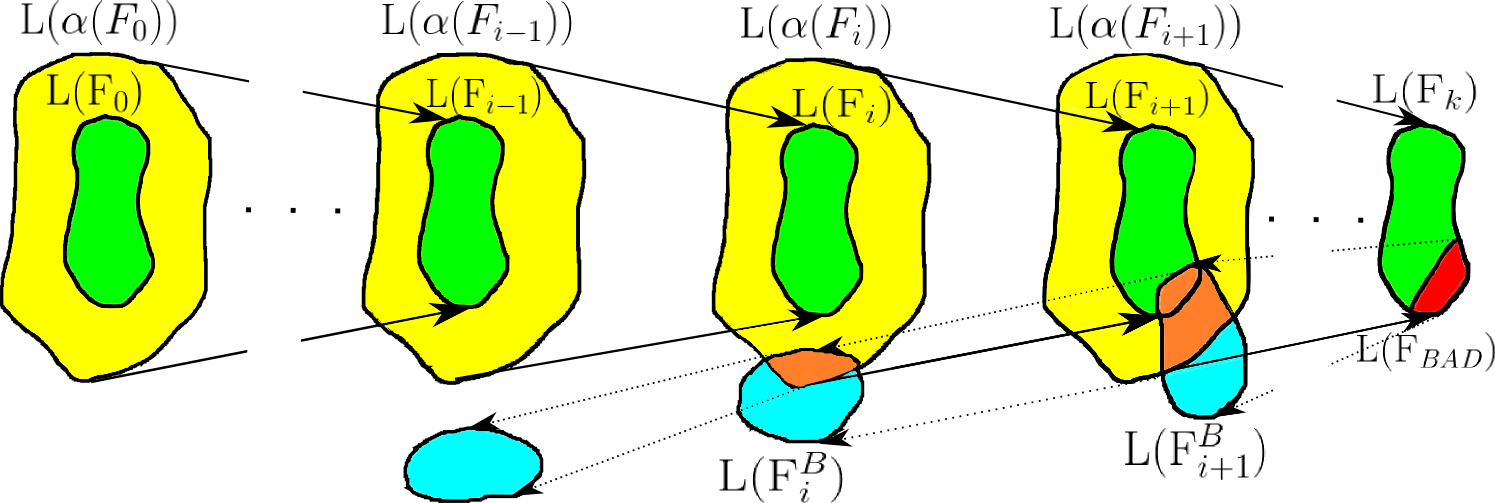
\includegraphics[scale=0.2]{artmc.png}
	\end{figure}

\end{frame}

%*******************************************************************************

%*******************************************************************************
\begin{frame}
\frametitle{Counterexample-guided Refinement of Abstraction}

	\begin{itemize}
		\item \hlgr{Ingredients for CEGAR}
		\begin{itemize}
			\item Forward run (already described)
			\item Backward run
			\item Abstraction refinement
		\end{itemize}
		\item \hlgr{Ingredients for backward run}:
		\begin{itemize}
			\item Reversion of abstract transformations
			\item Reversion of folding and unfolding boxes
			\item Reversion of abstraction $\leftarrow$ intersection of forest automata
				from backward run
		\end{itemize}
	\end{itemize}

\end{frame}

%*******************************************************************************

%*******************************************************************************
\begin{frame}
\frametitle{Reverting Abstract Transformers}
	\hlrd{Reversing forward run transformations}
	\begin{itemize}
		\item \hlbl{\texttt{x := malloc()}}\,--\,Removing created TA in forward run from FA
		\item \hlbl{\texttt{x := y->next}}\,--\,The $x$ variable is mapped to the value it has
			before this operation in forward run
		\item \hlbl{\texttt{free(x)}}\,--\,Removed TA in forward run is returned to FA
		\item \hlbl{\texttt{x == y}}\,--\,Has no reverse semantics.
	\end{itemize}

	\hlrd{Folding and unfolding of boxes}
	\begin{itemize}
		\item Reverting \hlbl{folding} of boxes by unfolding the box
			in backward run
		\item Reverting \hlbl{unfolding} of boxes by folding the box
			in backward
		\item By correct reverting we get so called \hlbl{compatible form}
			enabeling simplier bottom-up intersection of forest automata
	\end{itemize}

\end{frame}

%*******************************************************************************

%*******************************************************************************
\begin{frame}
\frametitle{Intersection of Forest Automata}
	\begin{itemize}
		\item Reverting abstraction over forest automaton
		\item \hlgr{Input:}
			\begin{itemize}
				\item FA \hlrd{$F_F=(A_1, \ldots, A_n, \sigma)$} from forward run before abstraction
			    \item FA \hlrd{$F_B=(B_1,\ldots, B_n, \sigma)$} from the backward run in the abstraction point
			\end{itemize}
		\item \hlgr{Preconditions:}
			\begin{itemize}
				\item Automata are in so called \hlbl{compatible form}\,---\,they
					have same number of TA with the same boxes in the corresponding transitions 
				\item Both FA have same $\sigma$\,---\,reversion of all operations precisely
			\end{itemize}

		\item \hlgr{Method:}
			\begin{itemize}
				\item Perform the intersection \hlbl{component-wise:} \hlrd{$F_F \cap F_B = (A_1 \cap A_n,\ldots,A_n\cap B_n, \sigma)$}
				\item When TA intersection reaches boxes in the transitions of both automata it calls the whole
					procedure for \hlbl{FA intersection recursively on the boxes} and uses its results as a new box
				\item If the intersection automaton has an empty language, derive predicates and restart the analysis.
					Otherwise, continue in backward run. 
			\end{itemize}
	\end{itemize}
\end{frame}

%*******************************************************************************

%*******************************************************************************
\begin{frame}
\frametitle{Predicates Derivation for Abatraction Refinement}

	\begin{itemize}
		\item Recall $F_A$ and $F_B$ from the previous slide
		\item When the intersection of FA is empty, the new predicates are derived
			from the FA $F_B$ of backward run
		\item Predicates are represented TA of $F_B$ such that \hlbl{TA $B_i$ is added
			to set of predicates $F_A$ if TA $A_i \cap B_i$ has an empty language}
		\item Refinement guarantees that the spurious counterexample will not
			be reached again with the same path
	\end{itemize}

\end{frame}
%*******************************************************************************

%*******************************************************************************
\begin{frame}
\frametitle{Experimental Evaluation}

	\begin{center}
	\hlbl{Results of experiments}
	\\~\\
	\begin{adjustbox}{max height=\textheight, max width=\textwidth}
	%\tiny
	%\caption{Results of experiments.}
	\begin{tabular}{| l | l | r | r | r | r || l | l | r | r | r | r | r |}
        \hline
		Program & Status & LoC & Time [s] & Refnm& Preds & Program & Status & LoC & Time [s] & Refnm & Preds \\
        \hline
        \hline
		SLL (delete) & \safe & $33$ & $0.02$ &  $0$ & $0$ & DLL (rev) & \safe & $39$ &  $0.70$ & $0$  & $0$ \\
        \hline
		SLL (bubblesort) & \safe & $42$ & $0.02$ &  $0$ & $0$ & CDLL & \safe & $32$ &  $0.02$  & $0$  & $0$ \\
        \hline
		SLL (insersort) & \safe & $36$ & $0.04$ & $0$ & $0$ & DLL (insersort) & \safe & $42$ &  $0.56$  & $0$  & $0$ \\
        \hline
		SLLOfCSLL & \safe & $47$ & $0.02$ & $0$ & $0$ & DLLOfCDLL & \safe & $54$ &  $1.76$  & $0$  & $0$ \\
        \hline
		\rowcolor{rowgray}
		\textbf{SLL01}    & \safe & $70$ & $1.20$   &  $1$ & $1$ & \textbf{DLL01} & \safe & $73$ &  $0.65$  & $2$  & $2$ \\
        \hline
		\rowcolor{rowgray}
		\textbf{CircularSLL} & \safe & $49$ & $3.57$   &  $3$  & $3$ & \textbf{CircularDLL} & \safe  & $52$ &  $37.22$ & $18$ & $24$ \\
        \hline
		\rowcolor{rowgray}
		\textbf{OptPtrSLL}   & \safe & $59$ & $1.90$ & $3$ & $3$ & \textbf{OptPtrDLL} & \safe & $62$ &  $1.87$  & $5$ & $5$ \\
        \hline
		\rowcolor{rowgray}
		\textbf{QueueSLL}    & \safe & $71$ & $11.32$  &  $10$ & $10$ & \textbf{QueueDLL} & \safe  & $74$ &  $44.68$ & $14$ & $14$ \\
		\rowcolor{rowgray}
        \hline
		\textbf{GBSLL}       & \safe & $64$ & $0.84$   &  $3$ & $3$ & \textbf{GBDLL} & \safe & $71$ &  $1.89$  & $4$ & $4$ \\
        \hline
		\rowcolor{rowgray}
		\textbf{GBSLLSent}   & \safe  & $68$ & $0.85$   &  $3$ & $3$ & \textbf{GBDLLSent} & \safe & $75$ &  $2.19$  & $4$ & $4$ \\
        \hline
		\rowcolor{rowgray}
		\textbf{RGSLL}       & \safe & $72$ & $14.41$  &  $22$  & $38$ & \textbf{RGDLL} & \safe & $76$ &  $78.76$ & $26$ & $26$ \\
        \hline
		\rowcolor{rowgray}
		\textbf{WBSLL}       & \safe & $62$ & $0.84$   &  $5$  & $5$ & \textbf{WBDLL} & \safe & $71$ &  $1.37$  & $7$ & $7$ \\
        \hline
		\rowcolor{rowgray}
		\textbf{SortedSLL}   & \safe & $76$ & $227.12$ &  $15$ & $15$ & \textbf{SortedDLL} & \safe & $82$ &  $36.67$ & $11$ & $11$ \\
        \hline
		\rowcolor{rowgray}
		\textbf{EndSLL}      & \safe  & $45$ & $0.07$   &  $2$  & $2$ & \textbf{EndDLL} & \safe & $49$ &  $0.10$  & $3$ & $3$ \\
        \hline
		\rowcolor{rowgray}
		\textbf{TreeRB} & \unsafe & $130$ &  $0.08$  & $0$  & $0$ & \textbf{TreeWB} & \unsafe & $125$ &  $0.05$  & $0$ & $0$ \\
        \hline
		TreeCnstr & \safe & $52$ & $0.31$  & $0$  & $0$ & \cellcolor{rowgray}\textbf{TreeCnstr} & \cellcolor{rowgray}\unsafe & \cellcolor{rowgray} $52$ & \cellcolor{rowgray} $0.03$  & \cellcolor{rowgray} $0$ & \cellcolor{rowgray} $0$ \\
        \hline
		TreeOfCSLL & \safe & $109$ &  $0.57$  & $0$  & $0$ & \cellcolor{rowgray}\textbf{TreeOfCSLL}  & \cellcolor{rowgray}\unsafe & \cellcolor{rowgray} $109$ & \cellcolor{rowgray} $0.56$  & \cellcolor{rowgray} $1$ & \cellcolor{rowgray} $3$ \\
        \hline
		TreeStack & \safe & $58$ &  $0.20$  & $0$  & $0$ & \cellcolor{rowgray}\textbf{TreeStack} & \cellcolor{rowgray}\unsafe & \cellcolor{rowgray} $58$ & \cellcolor{rowgray} $0.01$  & \cellcolor{rowgray} $0$ & \cellcolor{rowgray} $0$ \\
        \hline
		TreeDsw   & \safe & $72$ & $1.87$  & $0$  & $0$ & \cellcolor{rowgray}\textbf{TreeDsw} & \cellcolor{rowgray}\unsafe & \cellcolor{rowgray} $72$ & \cellcolor{rowgray} $0.02$  & \cellcolor{rowgray} $0$ &  \cellcolor{rowgray} $0$ \\
		\hline
		TreeRootPtr & \safe & $62$ &  $1.43$  & $0$  &  $0$ & \cellcolor{rowgray}\textbf{TreeRootPtr} & \cellcolor{rowgray}\unsafe & \cellcolor{rowgray} $62$ & \cellcolor{rowgray} $0.17$  & \cellcolor{rowgray} $2$ & \cellcolor{rowgray} $6$\\
        \hline
		SkipList    & \safe & $84$ & $3.36$  & $0$  & $0$ & \cellcolor{rowgray}\textbf{SkipList} & \cellcolor{rowgray}\unsafe & $\cellcolor{rowgray} 84$ & \cellcolor{rowgray} $0.08$  & \cellcolor{rowgray} $1$  & \cellcolor{rowgray} $1$ \\
        \hline
		% SkipList-3nd    & $97$ & $0.17$  & $1$  & N & x & $1$ & & & & & & & \\
        % \hline
	\end{tabular}
	\label{tab:times}
	\end{adjustbox}	
  % \vspace{-4mm}
  % \vspace{-8mm}
%\end{table}
	\end{center}

\end{frame}
%*******************************************************************************

%*******************************************************************************

\begin{frame}
  \frametitle{Conclusions}

  \begin{itemize}
	  \item \hlbl{Contribution:} Enable analysis of a new class of data structures\,---\,with relation
		  between nodes
		\item Designed backward run and predicate analysis for shape analysis based on forest automata 
		\item Designed compatible form and intersection of forest automata
		\item Experimentally evaluated on number of test cases
		\item \hlgr{Future work:}
			\begin{itemize}
				\item Find out reasons of state explosions on complicated tree structures
				\item Save Forest(er)!
			\end{itemize}
  \end{itemize}
\end{frame}

\end{document}
